\section{Repositório da Aplicação}

\label{section:repositorio-aplicacao}

Nessa seção do capítulo, apresenta-se o repositório da aplicação, que contém todos os arquivos relevantes ao projeto (como código-fonte, documentos e diagramas).

\subsection{Definição do repositório da aplicação}

Baseado na familiaridade dos integrantes em utilizar o sistema de controle de versão Git \cite{git-2025}, escolheu-se o GitHub \cite{github-2025} para hospedar o repositório remoto da aplicação e tornar o desenvolvimento mais colaborativo.

Visando garantir um repositório organizado e eficiente, estabeleceu-se uma estrutura de diretórios separando código-fonte da documentação do projeto e adotou-se o modelo de fluxo de trabalho \textit{Git Flow} \cite{gitflow-2023} para organizar o versionamento de ramificações. Além disso, foi utilizado \textit{Conventional Commits} \cite{convcommits-2025} para padronizar as mensagens de \textit{commit}, conferindo ainda mais organização.

\subsubsection{Link do repositório e especificações para acesso}

O \emph{QR Code} da Figura~\ref{fig:qrcode-repositorio} contém o link que leva diretamente ao repositório remoto do projeto hospedado no \emph{GitHub}. É possível tanto escanear quanto clicar no código abaixo para acessar o repositório.

\begin{figure}[h]
	\centering
		\caption{\emph{QR Code} do repositório da aplicação}
		\label{fig:qrcode-repositorio}
	\scalebox{1.5}{\qrcode{https://github.com/Henrriky/bs-beauty}}
	\fonte{Produzido pelos autores}
\end{figure}

Acessado o repositório, será aberta uma guia no navegador contendo uma página semelhante à Figura \ref{fig:inicio-repositorio}. Todos os arquivos do projeto podem ser visualizados diretamente pelo navegador. Como o repositório é público, qualquer pessoa pode acessá-lo e cloná-lo localmente usando \gls{https}. Para tanto, é necessário seguir as seguintes etapas:
 
\begin{enumerate}
	\item Instalar o Git na máquina (caso não esteja instalado).
	\item Escolher o diretório no qual o repositório será clonado.
	\item Abrir o terminal e alterar o diretório atual para o diretório escolhido.
	\item Usar o comando ``\texttt{git clone https://github.com/Henrriky/bs-beauty}''.
	\item Usar o comando ``\texttt{cd bs-beauty}'' para acessar o repositório clonado.
\end{enumerate}

\begin{figure}[h]
	\centering
	\caption{Página inicial do repositório}
	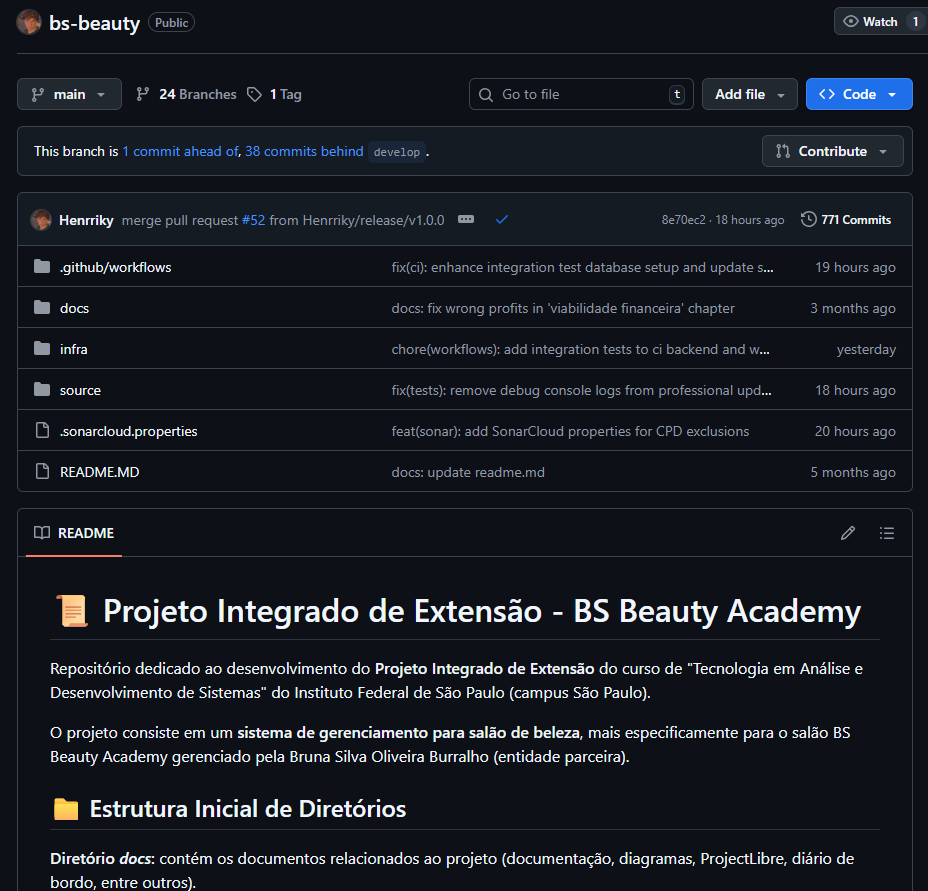
\includegraphics[width=0.8\textwidth]{cap03-gestao/imagens/bsbeauty-repositorio.png}
	\label{fig:inicio-repositorio}
	\fonte{Produzido pelos autores}
\end{figure}

Assim, o repositório estará devidamente clonado na máquina. Para execução local, utilize a \textit{branch} principal \texttt{main} e consulte o arquivo \texttt{README.MD} do repositório, que contém instruções de instalação de dependências e execução do projeto.

Para utilizar outros métodos de clonagem (como \gls{ssh}, \emph{GitHub} \gls{cli} ou baixar o arquivo \texttt{.zip} do projeto), consulte a documentação oficial do \emph{GitHub} \cite{clone-2025} referente às formas de clonar um repositório.